\section{Exploratory Data Analysis}
\label{sec:eda}

An exploratory data analysis was performed to characterize the NERMuD 2023 dataset beyond the basic split counts presented in Section~\ref{sec:dataset}. The analysis focuses on three aspects that are relevant for interpreting model performance: the imbalance between domains, the distribution of entity types, and the length of the input sequences.

\subsection{Domain Imbalance}
\label{subsec:eda-domain}

As shown in Table~\ref{tab:dataset-splits}, the three domains are not equally represented. Wikinews and fiction contain substantially more samples than the ADG domain, both in training and in test data. This imbalance is relevant when interpreting model performance: results on the smaller ADG domain may be influenced by the lower number of training examples, and a model that performs well on WN and FIC is not necessarily equally effective on ADG.

\subsection{Entity Distribution}
\label{subsec:eda-entities}

The dataset contains three entity types: persons (PER), organizations (ORG), and locations (LOC). Figure~\ref{fig:entity-distribution} presents the number of entities of each type across the splits. Person entities are the most frequent in the training set, followed by locations and organizations, and all three categories are represented in substantial numbers. The distribution is reasonably consistent across splits, ensuring that all entity types are represented in the development and test sets.

\begin{figure}[H]
    \centering
    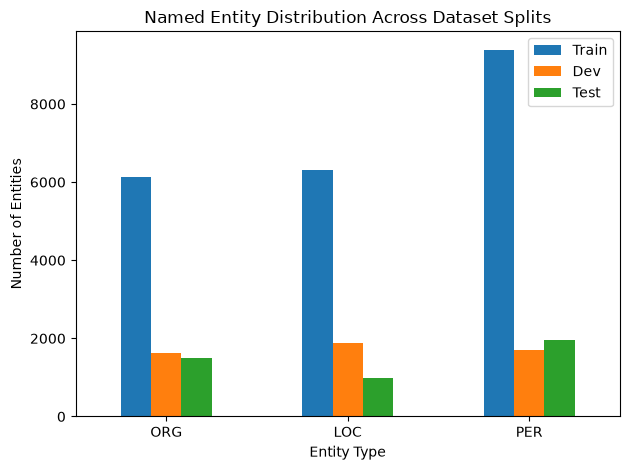
\includegraphics[width=0.65\textwidth]{figs/entity_distribution.png}
    \caption{Distribution of named entity types across dataset splits.}
    \label{fig:entity-distribution}
\end{figure}

The distribution of entity types also varies considerably across domains, as shown in Table~\ref{tab:entity-domain} for the training set. The FIC domain contains a notably high number of person entities but relatively few organization entities, whereas WN presents a more balanced distribution and the largest number of entities overall. These differences suggest that the domains place different demands on the models: a model trained mostly on fiction may be less exposed to organization entities, while a model trained on news may see a broader range of entity types.

\begin{table}[H]
    \centering
    \caption{Named entity distribution across domains in the training set.}
    \label{tab:entity-domain}
    \begin{tabular}{lrrr}
        \hline
        \textbf{Domain} & \textbf{LOC} & \textbf{ORG} & \textbf{PER} \\
        \hline
        ADG & 915  & 1,531 & 889 \\
        FIC & 587  & 137   & 3,177 \\
        WN  & 4,800 & 4,454 & 5,325 \\
        \hline
    \end{tabular}
\end{table}

\subsection{Sequence Length}
\label{subsec:eda-length}

The length of the input sequences was analyzed to determine an appropriate maximum sequence length for the experiments. Table~\ref{tab:sequence-length} presents descriptive statistics for the three splits.

\begin{table}[H]
    \centering
    \caption{Sequence length statistics in tokens.}
    \label{tab:sequence-length}
    \begin{tabular}{lrrr}
        \hline
        \textbf{Statistic} & \textbf{Train} & \textbf{Dev} & \textbf{Test} \\
        \hline
        Count  & 27,482 & 4,767 & 4,126 \\
        Mean   & 20.46 & 23.43 & 24.45 \\
        Std.   & 15.78 & 16.45 & 17.83 \\
        Min.   & 1 & 1 & 1 \\
        Median & 17 & 20 & 21 \\
        Max.   & 251 & 130 & 137 \\
        \hline
    \end{tabular}
\end{table}

Figure~\ref{fig:text-length} illustrates the distribution of sequence lengths. Most sequences are relatively short, with the majority concentrated well below the maximum observed length. The maximum length in the training set is 251 tokens, while the development and test sets reach 130 and 137 tokens, respectively. Based on these observations, a maximum sequence length of 256 tokens was selected for the Transformer models, providing sufficient capacity for the observed sequences while limiting unnecessary padding during training.

\begin{figure}[H]
    \centering
    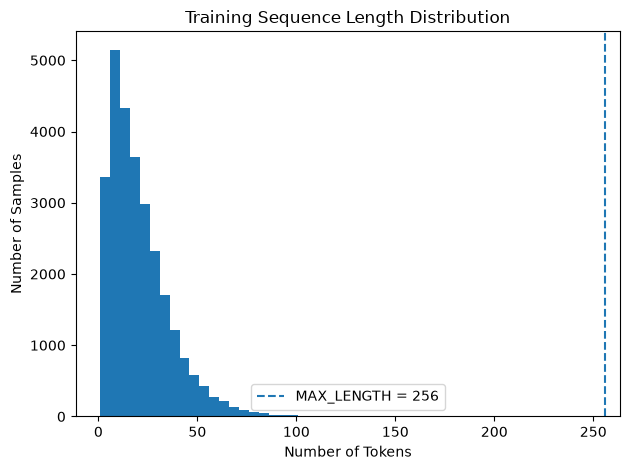
\includegraphics[width=0.7\textwidth]{figs/text_length_distribution.png}
    \caption{Distribution of sequence lengths in the NERMuD 2023 dataset.}
    \label{fig:text-length}
\end{figure}

\section{Model Training}
\label{sec:train}

Both models were fine-tuned for token-level classification using the Hugging Face \texttt{Transformers} library \cite{wolf2020transformers}. The training procedure was kept as similar as possible between the two models, so that differences in performance can be attributed mainly to the pretrained representations rather than to the training setup.

\subsection{Training Configuration}
\label{subsec:train-config}

The same hyperparameters were used for both models, including the effective batch size. Table~\ref{tab:train-config} summarizes the configuration, and the paragraphs below explain the rationale behind each choice.

\begin{table}[H]
    \centering
    \caption{Training configuration for UmBERTo and XLM-RoBERTa.}
    \label{tab:train-config}
    \begin{tabular}{lll}
        \hline
        \textbf{Parameter} & \textbf{UmBERTo} & \textbf{XLM-RoBERTa} \\
        \hline
        Max sequence length & 256 & 256 \\
        Learning rate & $2 \times 10^{-5}$ & $2 \times 10^{-5}$ \\
        Per-device batch size & 8 & 1 \\
        Gradient accumulation & -- & 8 \\
        Effective batch size & 8 & 8 \\
        Epochs & 3 & 3 \\
        Weight decay & 0.01 & 0.01 \\
        Optimizer & AdamW & AdamW \\
        Mixed precision (fp16) & No & Yes \\
        Random seed & 42 & 42 \\
        \hline
    \end{tabular}
\end{table}

\textbf{Maximum sequence length.} A maximum sequence length of 256 tokens was selected based on the exploratory analysis in Section~\ref{subsec:eda-length}, which showed that virtually all sequences in the dataset fall below this limit. This value provides sufficient capacity for the observed sequences while limiting the amount of unnecessary padding during training.

\textbf{Learning rate and weight decay.} A learning rate of $2 \times 10^{-5}$ and a weight decay of 0.01 follow common practices for fine-tuning Transformer models on token-classification tasks \cite{devlin2019bert}. Smaller learning rates are typically used for fine-tuning than for training from scratch, because the pretrained weights already encode useful representations that should not be destroyed by large updates.

\textbf{Effective batch size.} Both models were trained with an effective batch size of 8. UmBERTo fits a per-device batch size of 8 directly in GPU memory. XLM-RoBERTa, however, has a much larger vocabulary (250,002 tokens, compared to 32,005 for UmBERTo), which increases the memory required for the embedding layer and the classifier. To keep the effective batch size comparable, XLM-RoBERTa was trained with a per-device batch size of 1 and gradient accumulation over 8 steps. This means that gradients are accumulated over 8 forward passes before each optimizer update, producing an update equivalent to a batch of 8 examples.

\textbf{Mixed precision.} Mixed-precision training (\texttt{fp16}) was enabled for XLM-RoBERTa to reduce memory usage and speed up training on GPU. For UmBERTo, \texttt{fp16} was left disabled, since the model trained comfortably with full precision and the smaller vocabulary did not require the additional memory savings.

\textbf{Number of epochs.} Three epochs were used for both models. This value was chosen as a compromise between underfitting (too few epochs) and overfitting (too many epochs on a relatively small dataset), and the development set was used to verify that no clear overfitting occurred.

\textbf{Optimizer.} The AdamW optimizer, which is the default in the Hugging Face \texttt{Trainer}, was used for both models. AdamW decouples weight decay from the gradient update, which generally leads to better generalization than standard Adam.

\textbf{Random seed.} The random seed was fixed to 42 at the beginning of each notebook, controlling weight initialization, data shuffling, and dropout, which improves the reproducibility of the experiments. The \texttt{data\_seed} argument was also set to 42 for XLM-RoBERTa to ensure that data shuffling is reproducible independently of the model seed.

\subsection{Training Dynamics}
\label{subsec:train-dynamics}

The development set was evaluated after every epoch, and the checkpoint with the highest development F1-score was retained for final evaluation. Table~\ref{tab:dev-f1} reports the development F1-score obtained by each model at the end of each epoch.

\begin{table}[H]
    \centering
    \caption{Development F1-score after each training epoch.}
    \label{tab:dev-f1}
    \begin{tabular}{lccc}
        \hline
        \textbf{Model} & \textbf{Epoch 1} & \textbf{Epoch 2} & \textbf{Epoch 3} \\
        \hline
        UmBERTo & 0.8602 & 0.8724 & \textbf{0.8834} \\
        XLM-RoBERTa & 0.8070 & 0.8359 & \textbf{0.8519} \\
        \hline
    \end{tabular}
\end{table}

Both models improved steadily across the three epochs, and the best development F1-score was obtained in the final epoch in both cases. This suggests that additional epochs could potentially yield further gains, although the improvement between the second and third epochs was already smaller than between the first and the second, indicating that the models were approaching convergence.

Training time differed substantially between the two models. UmBERTo completed three epochs in approximately 18 minutes, whereas XLM-RoBERTa required 1 hour and 11 minutes under the gradient-accumulation and mixed-precision setting described above. This difference reflects both the larger vocabulary of XLM-RoBERTa and the additional forward passes required by gradient accumulation.

The comparison between the two models is fair with respect to the optimization regime: both were trained with the same effective batch size (8), the same learning rate, the same number of epochs, the same data splits, and the same evaluation procedure. Gradient accumulation was used for XLM-RoBERTa so that its effective batch size matches that of UmBERTo, despite the smaller per-device batch size required by its larger vocabulary.

However, the comparison does not control for every possible factor. The two models differ not only in pretraining language coverage but also in tokenizer vocabulary, pretraining corpus, and pretraining objective. Part of the observed difference in performance may therefore be attributable to these factors rather than to the language coverage of the pretraining data alone. The results should be interpreted as a comparison between two specific pretrained checkpoints under a shared training protocol, rather than as a controlled experiment isolating the effect of language-specific pretraining.

\subsection{Implementation}
\label{subsec:train-impl}

Training was implemented using the Hugging Face \texttt{Trainer} API. The model, tokenizer, data collator, and evaluation metrics were configured through small utility modules (\texttt{config.py}, \texttt{data\_utils.py}, \texttt{metrics.py}, and \texttt{models\_utils.py}) so that both models are trained with the same code path.

Token-level labels were aligned with subword tokens using the standard \texttt{word\_ids} strategy: the first subword of each word receives the original BIO label, while the remaining subwords and special tokens are assigned the label \texttt{-100} and ignored by the loss function \cite{devlin2019bert}. This ensures that the model is trained on word-level entity boundaries rather than on arbitrary subword fragments.

\section{Model Evaluation}
\label{sec:eval}

\section{Discussion}
\label{sec:disc}

